% CFA模型模板
% 验证性因子分析

\documentclass{standalone}
\usepackage{tikz}
\usetikzlibrary{shapes, arrows.meta, positioning}

% TikZ样式定义
\tikzstyle{latent} = [ellipse, draw, minimum width=2cm, minimum height=1cm]
\tikzstyle{manifest} = [rectangle, draw, minimum width=1.5cm, minimum height=0.8cm]
\tikzstyle{error} = [circle, draw, minimum size=0.6cm]
\tikzstyle{reg} = [->, >=stealth]

\begin{document}

% ============================================================================
% 单因子CFA
% ============================================================================

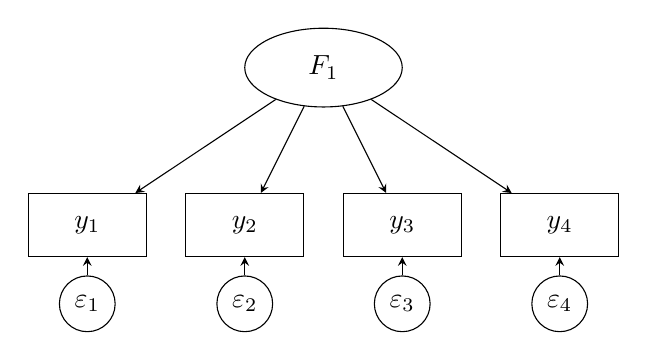
\begin{tikzpicture}
  % 潜变量
  \node[latent] (F1) at (0,2) {$F_1$};
  
  % 观测变量
  \node[manifest] (y1) at (-3,0) {$y_1$};
  \node[manifest] (y2) at (-1,0) {$y_2$};
  \node[manifest] (y3) at (1,0) {$y_3$};
  \node[manifest] (y4) at (3,0) {$y_4$};
  
  % 误差项
  \node[error] (e1) at (-3,-1) {$\varepsilon_1$};
  \node[error] (e2) at (-1,-1) {$\varepsilon_2$};
  \node[error] (e3) at (1,-1) {$\varepsilon_3$};
  \node[error] (e4) at (3,-1) {$\varepsilon_4$};
  
  % 路径
  \draw[reg] (F1) -- (y1);
  \draw[reg] (F1) -- (y2);
  \draw[reg] (F1) -- (y3);
  \draw[reg] (F1) -- (y4);
  
  \draw[reg] (e1) -- (y1);
  \draw[reg] (e2) -- (y2);
  \draw[reg] (e3) -- (y3);
  \draw[reg] (e4) -- (y4);
\end{tikzpicture}

% ============================================================================
% 多因子CFA
% ============================================================================

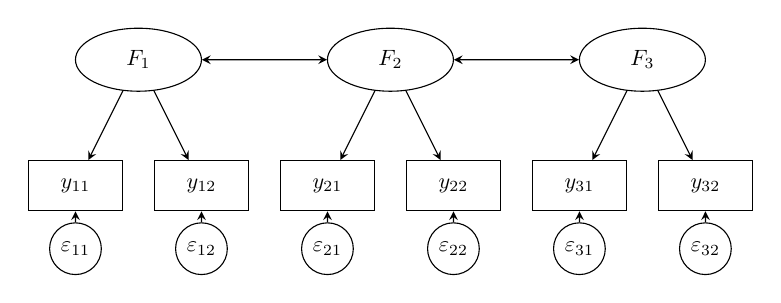
\begin{tikzpicture}[scale=0.8, transform shape]
  % 潜变量
  \node[latent] (F1) at (0,2) {$F_1$};
  \node[latent] (F2) at (4,2) {$F_2$};
  \node[latent] (F3) at (8,2) {$F_3$};
  
  % F1的指标
  \node[manifest] (y11) at (-1,0) {$y_{11}$};
  \node[manifest] (y12) at (1,0) {$y_{12}$};
  
  % F2的指标
  \node[manifest] (y21) at (3,0) {$y_{21}$};
  \node[manifest] (y22) at (5,0) {$y_{22}$};
  
  % F3的指标
  \node[manifest] (y31) at (7,0) {$y_{31}$};
  \node[manifest] (y32) at (9,0) {$y_{32}$};
  
  % 误差项
  \node[error] (e11) at (-1,-1) {$\varepsilon_{11}$};
  \node[error] (e12) at (1,-1) {$\varepsilon_{12}$};
  \node[error] (e21) at (3,-1) {$\varepsilon_{21}$};
  \node[error] (e22) at (5,-1) {$\varepsilon_{22}$};
  \node[error] (e31) at (7,-1) {$\varepsilon_{31}$};
  \node[error] (e32) at (9,-1) {$\varepsilon_{32}$};
  
  % 路径
  \draw[reg] (F1) -- (y11);
  \draw[reg] (F1) -- (y12);
  \draw[reg] (F2) -- (y21);
  \draw[reg] (F2) -- (y22);
  \draw[reg] (F3) -- (y31);
  \draw[reg] (F3) -- (y32);
  
  \draw[reg] (e11) -- (y11);
  \draw[reg] (e12) -- (y12);
  \draw[reg] (e21) -- (y21);
  \draw[reg] (e22) -- (y22);
  \draw[reg] (e31) -- (y31);
  \draw[reg] (e32) -- (y32);
  
  % 潜变量协方差
  \draw[<->, >=stealth] (F1) -- (F2);
  \draw[<->, >=stealth] (F2) -- (F3);
\end{tikzpicture}

% ============================================================================
% 二阶因子模型
% ============================================================================

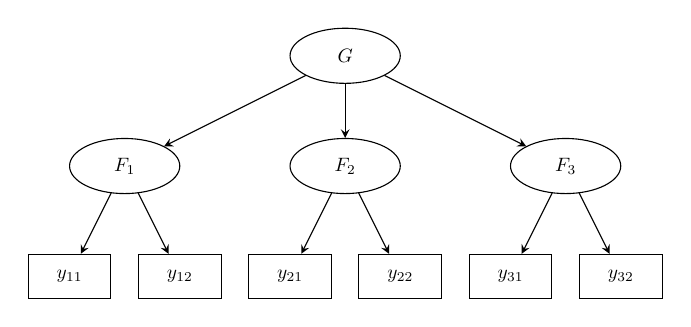
\begin{tikzpicture}[scale=0.7, transform shape]
  % 二阶潜变量
  \node[latent] (G) at (4,4) {$G$};
  
  % 一阶潜变量
  \node[latent] (F1) at (0,2) {$F_1$};
  \node[latent] (F2) at (4,2) {$F_2$};
  \node[latent] (F3) at (8,2) {$F_3$};
  
  % 指标
  \node[manifest] (y11) at (-1,0) {$y_{11}$};
  \node[manifest] (y12) at (1,0) {$y_{12}$};
  \node[manifest] (y21) at (3,0) {$y_{21}$};
  \node[manifest] (y22) at (5,0) {$y_{22}$};
  \node[manifest] (y31) at (7,0) {$y_{31}$};
  \node[manifest] (y32) at (9,0) {$y_{32}$};
  
  % 二阶因子载荷
  \draw[reg] (G) -- (F1);
  \draw[reg] (G) -- (F2);
  \draw[reg] (G) -- (F3);
  
  % 一阶因子载荷
  \draw[reg] (F1) -- (y11);
  \draw[reg] (F1) -- (y12);
  \draw[reg] (F2) -- (y21);
  \draw[reg] (F2) -- (y22);
  \draw[reg] (F3) -- (y31);
  \draw[reg] (F3) -- (y32);
\end{tikzpicture}

% ============================================================================
% 双因子模型
% ============================================================================

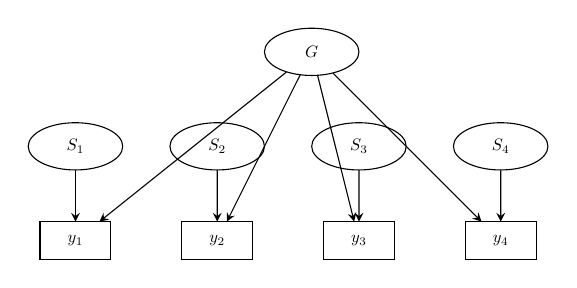
\begin{tikzpicture}[scale=0.6, transform shape]
  % General factor
  \node[latent] (G) at (5,3) {$G$};
  
  % Specific factors
  \node[latent] (S1) at (0,1) {$S_1$};
  \node[latent] (S2) at (3,1) {$S_2$};
  \node[latent] (S3) at (6,1) {$S_3$};
  \node[latent] (S4) at (9,1) {$S_4$};
  
  % 指标
  \node[manifest] (y1) at (0,-1) {$y_1$};
  \node[manifest] (y2) at (3,-1) {$y_2$};
  \node[manifest] (y3) at (6,-1) {$y_3$};
  \node[manifest] (y4) at (9,-1) {$y_4$};
  
  % General factor载荷
  \draw[reg] (G) -- (y1);
  \draw[reg] (G) -- (y2);
  \draw[reg] (G) -- (y3);
  \draw[reg] (G) -- (y4);
  
  % Specific factor载荷
  \draw[reg] (S1) -- (y1);
  \draw[reg] (S2) -- (y2);
  \draw[reg] (S3) -- (y3);
  \draw[reg] (S4) -- (y4);
\end{tikzpicture}

\end{document}
